\begin{center}
	\huge \textbf{Il modello PRNR}
	
	\rule{7cm}{0.4pt} 
	
	\LARGE Un modello matematico per la Rivoluzione Francese
	
	\vspace{20pt}
	
	\LARGE \textbf{Cristina Caprioglio, Luca Morelli}
	
	\vspace{5pt}
	
	\LARGE 20 Dicembre 2022
	
	\vspace{20pt}
 
	\normalsize\textbf{Abstract:}\\
\end{center}
Scrivere un Abstract.

\vspace{20pt}

\section*{Introduzione}
I modelli a compartimenti ... spiegare cosa sono e come funzionano
\section{Il sistema e il modello}
Vogliamo studiare la dinamica di una popolazione composta da vari membri, in numero elevato, che differiscono l'uno dall'altro per il loro reddito, queste differenze, sotto determinate condizioni, possono spingere alcuni individui ad insorgere, analogamente l'insurrezione di alcuni individui può essere repressa dai più abbienti tramite l'uso della forza.\\

Per modellizzare una popolazione eterogenea abbiamo deciso di suddividerla in due categorie, \textbf{Poveri} e \textbf{Nobili}, per le quali si considera un reddito medio caratteristico di ciascuna categoria.\\
Ogni membro di questa popolazione può decidere, in base a vari fattori, di far uso della violenza per far valere le esigenze della propria categoria. Abbiamo considerato che ogni individuo può trovarsi o in uno stato di normalità o in uno stato eccitato: un membro della categoria dei Poveri nello stato \textbf{Normale} $(N_P)$ può transire allo stato di \textbf{Rivoluzionario} $(R)$ mentre un membro della categoria dei Nobili nello stato \textbf{Normale} $(N_N)$ può transire allo stato di \textbf{Reazionario} $(\bar{R})$ e all'interno della stessa categoria può avvenire anche la transizione inversa, come mostrato in figura (\ref{fig:CompartmentScheme}).\\
\begin{figure}[H]
	\centering
	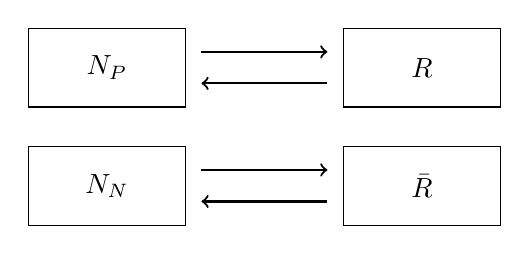
\begin{tikzpicture}
        \draw[draw=black] (0,0) rectangle (2,1);
		\draw[->, thick] (2.2,.7) -- (3.8,.7);
		\draw[<-, thick] (2.2,.3) -- (3.8,.3);
		\draw[draw=black] (4,0) rectangle (6,1) ;
		\node at (5,0.5) {$\bar{R}$};
		\node at (1,0.5) {$N_N$};
		\draw[draw=black] (0,1.5) rectangle (2,2.5);
		\draw[->, thick] (2.2,2.2) -- (3.8,2.2);
		\draw[<-, thick] (2.2,1.8) -- (3.8,1.8);
		\draw[draw=black] (4,1.5) rectangle (6,2.5) ;
		\node at (5,2) {$R$};
		\node at (1,2) {$N_P$};
    \end{tikzpicture}
	\label{fig:CompartmentScheme}
	\caption{Schema a compartimenti delle categorie delle persone. Con le frecce sono evidenziate le transizioni di stato che un individuo può effettuare.}
\end{figure}
Per questa modellizazione abbiamo deciso, come è consueto fare, di non  considerare le possibili fluttuazioni del numero totale di individui dovuti alla morte e alla nascita di persone, inoltre abbiamo considerato che un individuo non possa transire dalla categoria di Povero a quella di Nobile, questa scelta è giustificata dall'osservazione che seppur tali transizioni potrebbero avvenire in genere in genere sono estremamente rare. Queste considerazioni ci hanno permesso di identificare 3 vincoli da imporre al modello:
\begin{equation}
    \frac{N_P(t)+R(t)}{N_P(0)+R(0)+N_N(0)+\bar{R}(0)}=F_P \qquad\frac{N_N(t)+\bar{R}(t)}{N_P(0)+R(0)+N_N(0)+\bar{R}(0)}=F_N \qquad F_P+F_N=1 
	\label{vincoli}
\end{equation}
dove $F_P$ e $F_N$ sono rispettivamente le frazioni di individui Poveri e Nobili sulla popolazione totale.\\

Dobbiamo ora identificare quali equazioni regolino la dinamica del sistema, per questo abbiamo ragionevolmente supposto che:
\begin{itemize}
	\item un Povero possa transire allo stato di Rivoluzionario o di sua spontanea iniziativa per colpa della sua condizione di povertà oppure incontrando un rivoluzionario che lo convinca ad insorgere
	\item un Rivoluzionario incontrando dei Reazionari può essere convinto a non perseguire più la sua causa ritornando ad essere allo stato Normale
	\item un Nobile incontrando un rivoluzionario in risposta può decidere di diventare un Reazionario
	\item un Reazionario vedendo diminuire il numero di Rivoluzionari, e quindi aumentare quello di Poveri allo stato normale, può decidere di ritornare anch'esso allo stato normale  
\end{itemize}
Se consideriamo un tempo $\Delta t$ possiamo esprimere le variazioni del numero di ogni compartimento tenendo conto delle precedenti considerazioni:
\begin{flalign}
      &R(t+\Delta t)-R(t)=\Gamma N_P(t) R(t)\Delta t+\gamma N_P(t)\Delta t-\bar{\Gamma}R(t)\bar{R}(t)\Delta t\\\nonumber
	  &\bar{R}(t+\Delta t)-\bar{R}(t)=\alpha N_N(t)R(t)\Delta t-\beta \bar{R}(t)N_P(t)\Delta t\\\nonumber
	  &N_P(t+\Delta t)-N_P(t)=-(R(t+\Delta t)-R(t))\\\nonumber
	  &N_N(t+\Delta t)-N_N(t)=-(\bar{R}(t+\Delta t)-\bar{R}(t))\\\nonumber
\end{flalign}	
    